\begin{pagefigure}
\centering
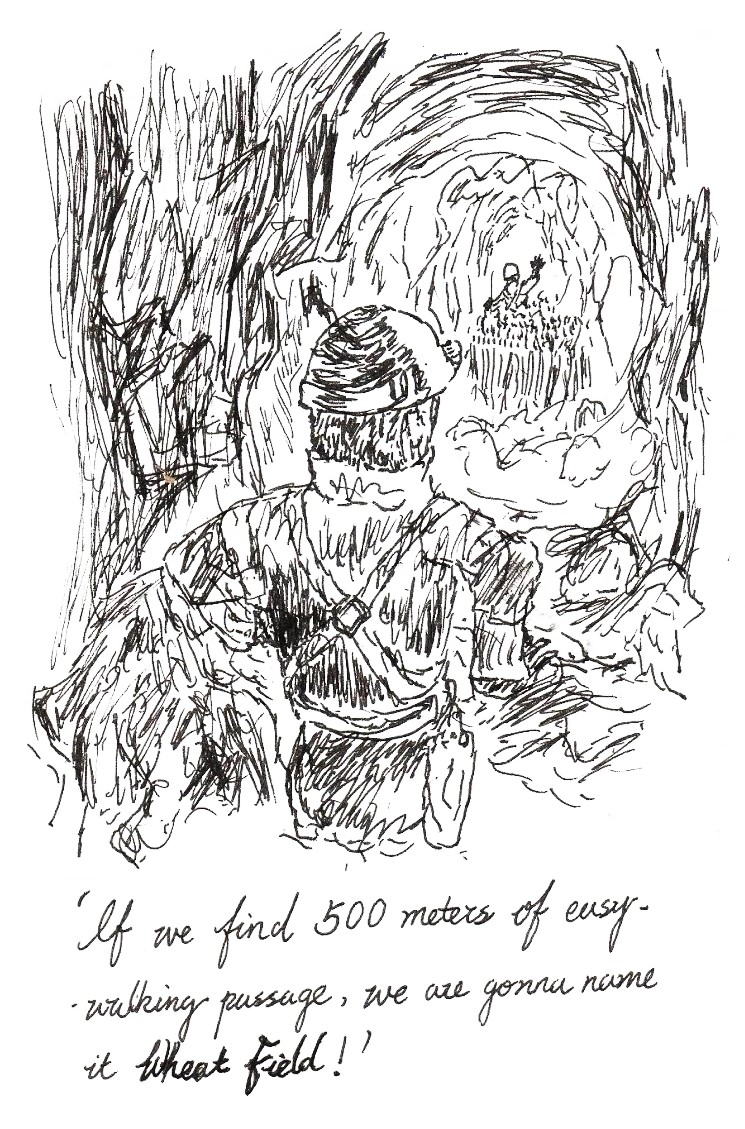
\includegraphics[width=0.9\linewidth]{images/overview/the_caver_2.jpg}
\caption{Drawn by Larry Jiyu Jiang}
\label{}
\end{pagefigure}
\newpage


\begin{tcolorbox} %makes a white opaque background for the text.
\vspace{60pt}
	\part{Introduction}
	\lettrine{S}{istem} \passage{Migovec}, tucked away at the western edge of the \passage{Triglavski Narodni Park} is the longest cave system in Slovenia.  It has held that title since 2012, when, defying expectations after a half a decade of effort, the connection between the `Old System' (\passage{M2}-\passage{M16}-\passage{M18}) and the newer \passage{Vrtnarija} (Gardeners' World) and \passage{Vilinska Jama} cave was forged after a routine pushing trip at -600\,m.

Thirty eight years after the first explorations underneath \passage{Tolminski Migovec}, or `Mig' as it is affectionately named, this connection made the national news. 

Since then, and rather more discreetly, Imperial College (ICCC) and Jamarska Sekcija PD Tolmin (JSPDT) cavers have repeatedly spent their part of their summers searching for more empty space under the Hollow Mountain. Bit by bit, other pieces of the puzzle were extended and connected to the main system.

In 2015, three Slovene cavers found a way between the \passage{Primadona}-\passage{Monatip}-\passage{Ubend571} cave system and one of the high level passages of \passage{Sistem Migovec}, bringing the sum total to 35.6km of interconnected passage. 

As of 2018, it stood at 39.2\,km, with, it is hoped, plenty more tales of exploration and adventure to come...


\end{tcolorbox}
	\backgroundsetup{	scale=1,
					color=black,
					opacity=1,
					angle=0,
					contents={%
							  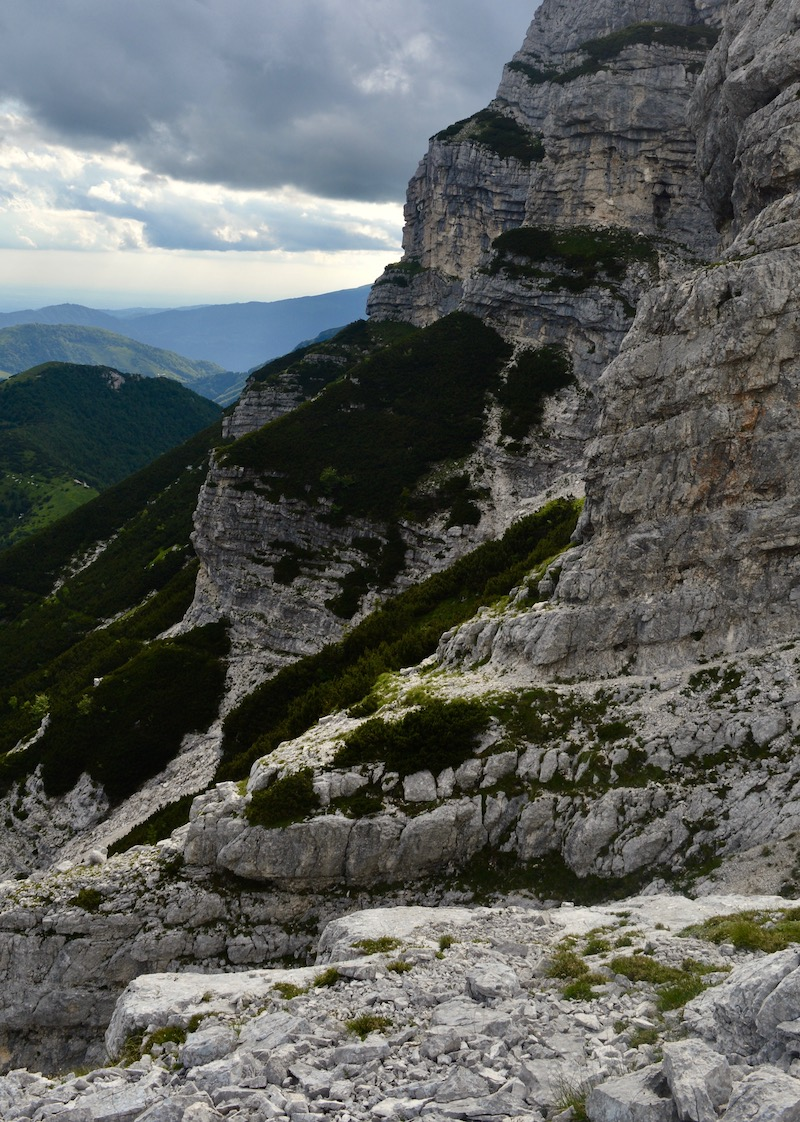
\includegraphics[height=\paperheight]{images/backgrounds/migface.jpg}
  					} % this puts the entire image as local background
	}
\BgThispage %calls the image to be displayed as background, flush with paper edge.
